

Figure \ref{fig:decompos} describes the decomposition of CPU usage based on trends, seasonality, levels, and residual (errors). Those attribute helps to understand time-series dataset and discover the pattern in a dataset that helps to forecast the future data. ‘statsmodels.tsa.seasonal’ package provides the decompose of a dataset which is mentioned in Figure \ref{fig:decompos} .
\begin{figure}
  \centering
    
      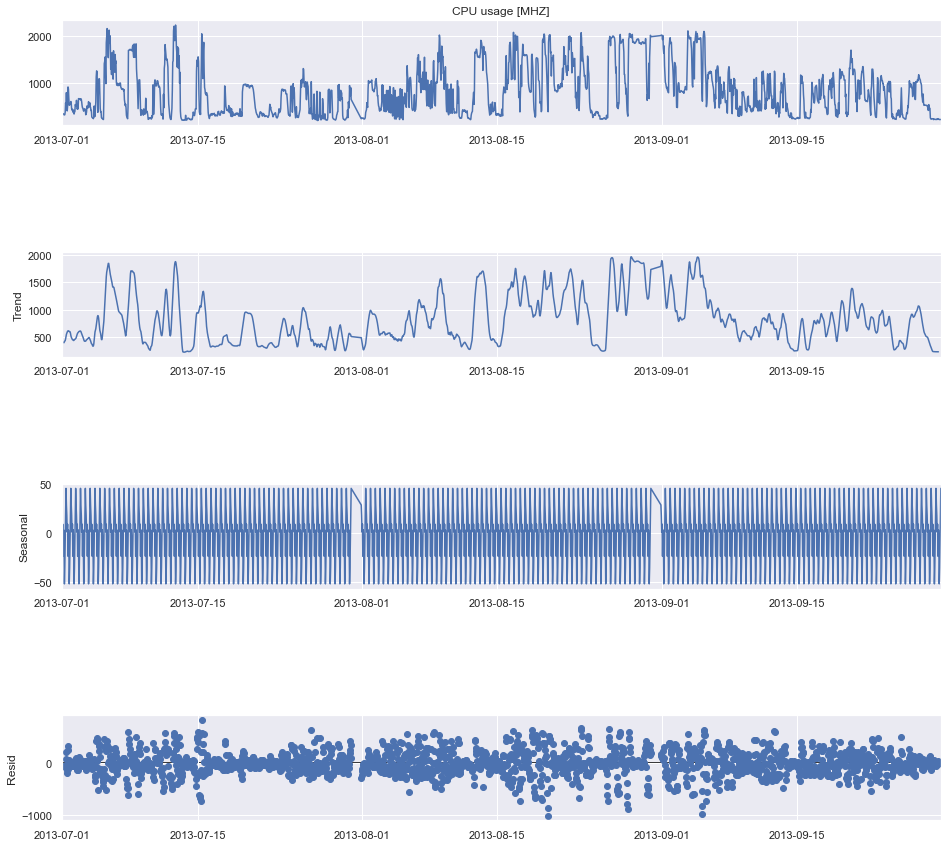
\includegraphics[width=1\textwidth]{decomposition.png}
  \caption{Decomposition of CPU usage data}
  \label{fig:decompos}
\end{figure}

\textbf{Data is Stationary or not?}

As mentioned in chapter 3, for time series analysis data should be in stationary form.
There is a number of tests are available to check data stationery or not.
\begin{enumerate}
\item Dicky-Fuller Test
\item KPSS test
\item The Zivot and Andrews Test 
\item Variance Ratio Test
\end{enumerate}

\textbf{Augmented Dicky-fuller Test}

Augmented Dicky-fuller test is the Unit root test which is normally used to check data is stationary or not. Unit Root test identifies all the characteristics in the time series data which makes it non-stationary. It performs an autoregression model to optimize the relevant information among different lag observations. ADF has two Hypothesis, one Null Hypothesis which derive from the unit root test and represent data is non-stationary, while the Alternate Hypothesis represents data is stationary (21).
The p-value in the ADF provides an interpretation of the result, if the p-value below the threshold i.e., 5\% or 1\% which makes the data stationary by rejecting Null Hypothesis. On the other side,  if your p-value is above the threshold i.e., (5\% or 1\%) which makes data Non-stationary. In python, the stats model package defines ‘adfuller()’ to perform the ADF test \cite{cheung1995lag}.After performing the ADF test on the BitBrain dataset, it concludes that attributes of a dataset (CPU usage, Memory usage, network transmitted throughput and Network received throughput) is stationary.

\section{ARIMA Model}

An ARIMA model first checks data is stationary using the ADF test which is mentioned above, after consideration above test pass through the ARIMA model. ARIMA model has 3 parameter (p, d, q). To hyper tuning parameter in the ARIMA model, there is one python package ‘pmdarima’ provide auto\_arima function that is very useful to select the optimal value of p,d,q. they compare AIC (Akaike information criterion) and the lowest score value of AIC choose to predict the ARIMA model. AIC is an error predictor which calculates the total number of information loss by the model if the AIC score is less then model is highly qualified for forecasting the result. Figure \ref{fig:score} mentioned above all possible combinations that perform on the ARIMA model and based on the AIC score choose optimal value of p,d,q. based on the result ARIMA model predict based on (2,0,3). Figure \ref{fig:arima} describes the result of ARIMA(2,0,3) model prediction with test data and based on error metrics RMSE error is 537.6187 and MAE score is 386.8786. good model RMSE score is less than 180 so the ARIMA model not effective to predict a good result.
\begin{figure}
  \centering
    
      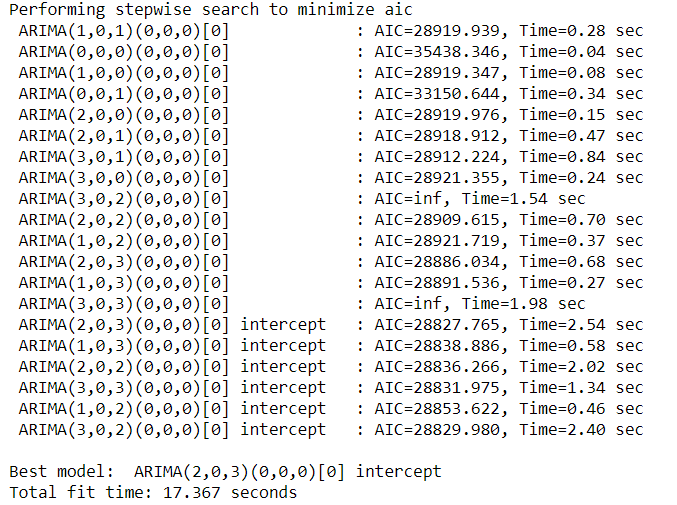
\includegraphics[width=1\textwidth]{AIC_SCORE_ARIMA.png}
  \caption{AIC score of auto\_arima function}
  \label{fig:score}
\end{figure}
\begin{figure}
  \centering
    
      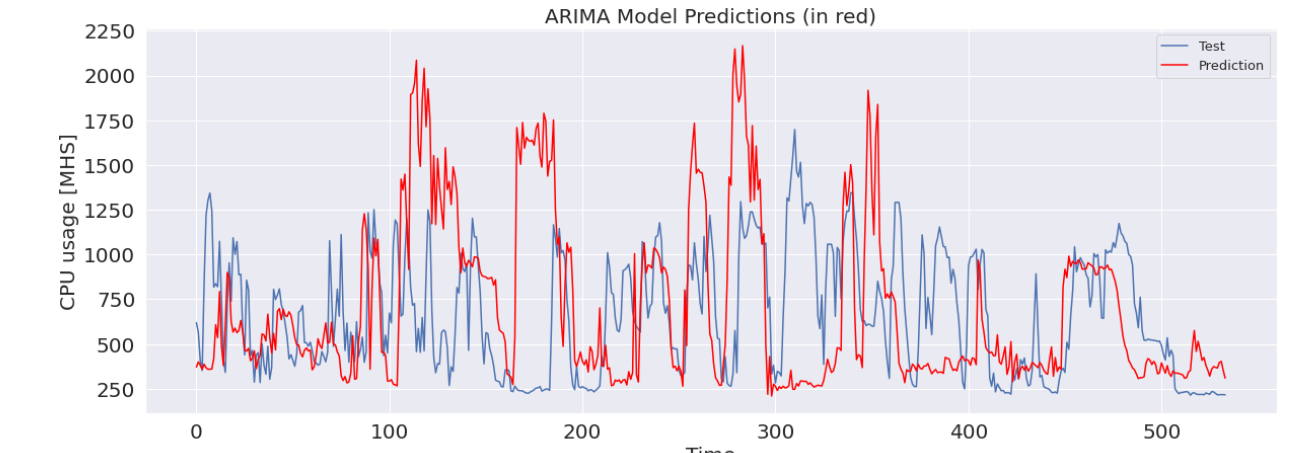
\includegraphics[width=1\textwidth]{ARIMA.png}
  \caption{Test vs Prediction model on ARIMA(2,0,3)}
  \label{fig:arima}
\end{figure}

\section{ Vector Auto Regression(VAR) Model}
VAR model normally used to predict multivariate time series, the dataset is divided into two parts 75\% as training data and remaining for testing a model. Before applying data to the model, first check data is stationary or not. VAR Model uses Augmented Dicky-Fuller(ADF) test to check the data is stationary or not. Parameter of dataset i.e. CPU usage, Memory Usage, Network Transmit throughput, Network received Throughput, is all stationary.

\begin{table}[h]
\caption{AIC score for lag values} %title of the table
\centering % centering table

\begin{tabular}{ m{5cm}  m{5cm}} % creating eight columns
\hline\hline %inserting double-line
 
lag order & AIC score\\
\hline\hline
1 & 70.7932\\
2 & 70.3678\\
3 & 70.1933 \\
4 & 70.0852  \\
5 & 69.9839 \\
6 & 69.9778 \\
7 & 69.9764 \\
8 & 69.9839 \\
9 & 70.0030 \\
10 & 70.0489 \\ [1ex]

\hline % inserts single-line
\hline % inserts single-line
\end{tabular}

\label{tab:aictab}
\end{table}

\begin{figure}
  \centering
    
      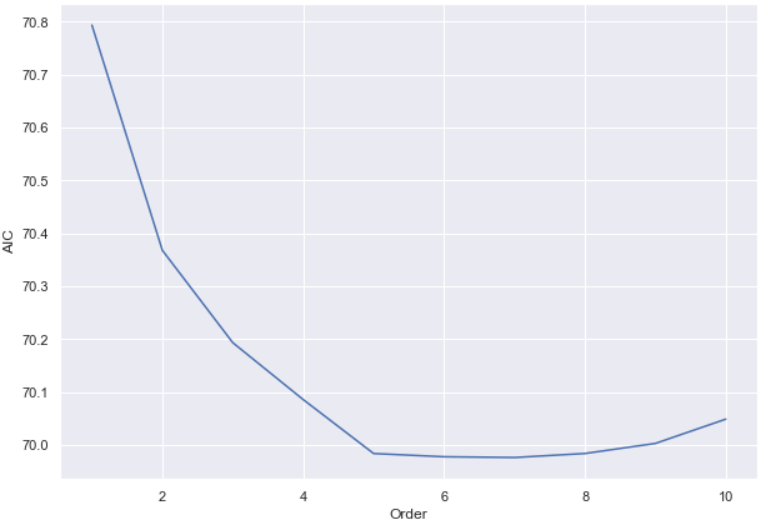
\includegraphics[width=1\textwidth]{VAR_AIC_CHART.png}
  \caption{lag order plot based on AIC score}
  \label{fig:aic}
\end{figure}

VAR model based on Auto Regression so to get optimal value of lag value, try max value of lag as a 10 and calculate AIC score which mentioned in 5.1. based on the lowest score of AIC select the lag value and pass it to the model.  Figure \ref{fig:aic} represents the AIC score and plot for the VAR model based on comparison select the lowest AIC score lag value to train the model. Using 7 lag value for p VAR model trained and predict the CPU cores with 0.2287 MAE error and 0.3538 RMSE error, for CPU usage 401.026 MAE error and 479.814 RMSE error, for memory usage  1633.6453 MAE and 1915.21 RMSE, for disk read throughput prediction error 34.775 MAE and 43.2363 RMSE, and, network received throughput error is 22.713 MAE and 33.23 RMSE with respect to BitBrain dataset.
